\begin{figure*}
	\centering
	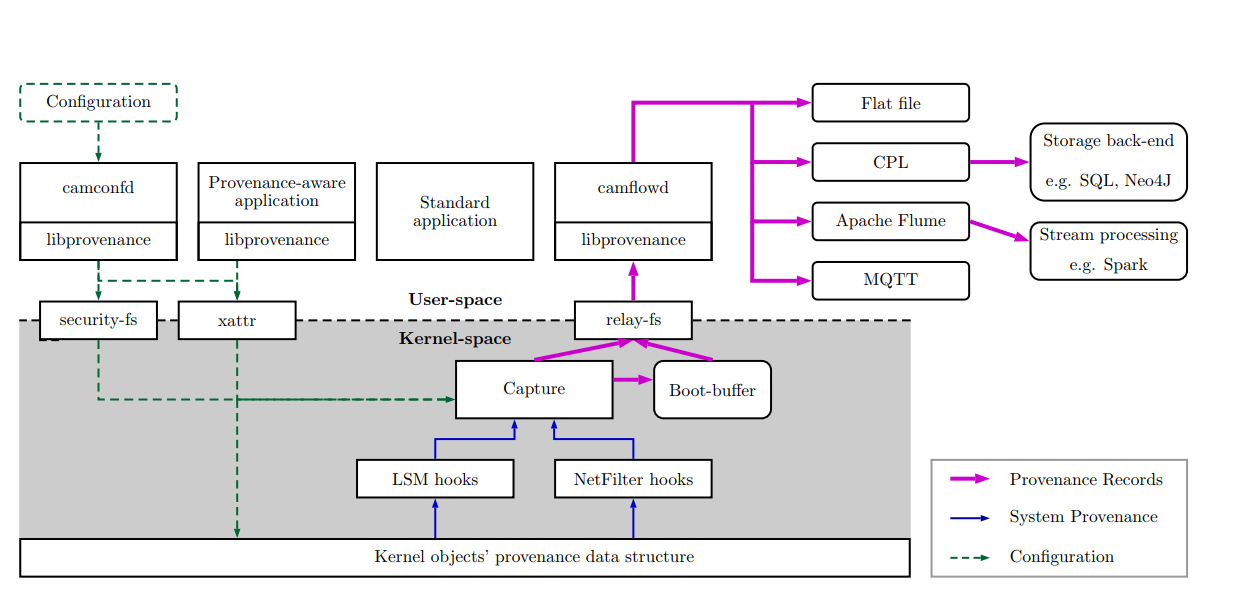
\includegraphics[width=0.7\linewidth]{camflow}
	\caption[Architecture overview]{Camflow architure}
	\label{fig:camflow}
\end{figure*}


\label{Introduction}
Though we have introduced what a Linux Security Module(LSM) means, we will discuss it in a little more detail. The Linux Security Module (LSM) framework provides a mechanism for various security checks to be hooked by new kernel extensions. The name “module” is a bit of a misnomer since these extensions are not actually loadable kernel modules. Instead, they are selectable at build-time via CONFIG\_DEFAULT\_SECURITY and can be overridden at boot-time via the "security=..." kernel command line argument, in the case where multiple LSMs were built into a given kernel.
\vskip 0.1in 
The primary users of the LSM interface are Mandatory Access Control (MAC) extensions which provide a comprehensive security policy. Examples include SELinux, Smack, Tomoyo, and AppArmor. In addition to the larger MAC extensions, other extensions can be built using the LSM to provide specific changes to system operation when these tweaks are not available in the core functionality of Linux itself.
\vskip 0.1in
Without a specific LSM built into the kernel, the default LSM will be the Linux capabilities system. Most LSMs choose to extend the capabilities system, building their checks on top of the defined capability hooks.





\section{Modeling the system calls causing flows}
The analysis technique we use if has been proposed by Georget et al. () for a subset of the system calls. It's a four step methodology which relies on the C compiler from the Gnu Compilers Collection(21). 

\begin{enumerate}
	\item The model designed by Georget to represent system calls and their execution paths does not describe the C source code. They instead use an internal representation called GIMPLE[]. 
	\item Each system call is represented by a control flow graph (CFG).
	\item The paths in these graphs model the execution paths in the program as defined by the classical graph theory[].
	\item The system calls are analysed one at a time. 
	\item Each system call contains multiple functions. These functions are inlined into the system calls to reduce the analysis to intra-procedural case. 
	\item Finally, in the CFGs, two kinds of nodes are marked: the nodes which correspond to the LSM hooks and the nodes which correspond to operation which generate the flows. 
	
\end{enumerate}

\subsection{Constraints in modelling}
In the CFGs which we construct , a node is not a basic block but a simple GIMPLE instruction. The analysis methodology does not deal with all expressions and variables of the language. Another reason for the same is that usage of floating-point values is explicitly prohibited in the Linux code. Variables representing structures or unions are also not handled when they involve pointer arithmetic. Global or volatile variables are also not handled, since they can have an arbitrary value at any point in the execution. Ignoring some variables does not hinder the soundness of
our approach: less impossible paths might be detected as such but
we never declare as impossible a possible path. A path in the CFG is said to be impossible when any execution
that would follow it would enter in an impossible state. For example,
a path including two conditional branching with incompatible
conditions would require a Boolean expression to be both true and
false at the same time. 


